\documentclass[12pt]{article}
\usepackage{graphicx}
\usepackage[utf8]{inputenc}
\usepackage[english]{babel}
\usepackage{fullpage}
\usepackage{listings}
\usepackage{xcolor}
\usepackage{url}
\usepackage[linesnumbered,ruled,vlined]{algorithm2e}
\usepackage{enumitem}
\usepackage{mathrsfs}
\usepackage{amssymb}
\usepackage{amsmath}
\usepackage{enumitem}
\usepackage{hyperref}
\usepackage{float}
\usepackage{sbc-template}


\definecolor{mygreen}{rgb}{0,0.6,0}

\hypersetup{
    colorlinks=true,
    linkcolor=cyan,
    urlcolor=cyan}

\newcounter{problem}
\newcounter{solution}

\pagestyle{plain}
\thispagestyle{plain}

\newtheorem{prop}{Proposição}
\newtheorem{ex}{Exemplo}[section]
\newtheorem{theorem}{Teorema}
\newtheorem{corollary}{Corolário}[theorem]
\newtheorem{lemma}[theorem]{Lemma}
\newtheorem{definition}{Definição}

\lstset{ % lstlisting
    language=Python,
    frame=tb, % draw a frame at the top and bottom of the code block
    tabsize=4, % tab space width
    showstringspaces=false, % don't mark spaces in strings
    commentstyle=\color{mygreen}, % comment color
    keywordstyle=\color{blue}, % keyword color
    stringstyle=\color{red}, % string color
    numbers=left, 
    numbersep=9pt,
    backgroundcolor=\color{black!5}, % set backgroundcolor
    basicstyle=\footnotesize,% basic font setting
}

\newcommand{\furl}[1]{\footnote{\url{#1}}}

\newcommand\Problem{%
  \stepcounter{problem}%
  \textbf{Problema \theproblem:}
  \setcounter{solution}{0}%
}

\newcommand\TheSolution{%
  \textbf{Solução:}\\%
}

\newcommand\ASolution{%
  \stepcounter{solution}%
  \textbf{Solução \thesolution:}\\%
}
% \parindent0in
\parskip 1.5em

\title{Curso de Curvas e Superfícies - Parte II}

\author{Wellington José Leite da Silva\inst{1}}

\address{Escola de Matemática Aplicada da FGV (EMAP), Brazil}

\date{}

\begin{comment}
http://150.164.25.15/~rodney/notas_de_aula/geometria_diferencial.pdf
\end{comment}

\begin{document}

\maketitle

\section*{Apresentação}\label{s1}
Continuando com o que foi construído na parte I apresentamos aqui uma linha de aprendizado do curso de curvas e superfícies apresentando definições, teoremas, exemplos, etc. Separados em \todo{Welly}{Adicionar as seções}. 

Com intuído de auxiliar o aprendizado aos tópicos apresentados e fornecer uma forma de visualização computacional apresentamos exemplos com códigos em \textit{SageMath}~\cite{sagemath}. Aqui seguimos o livro \cite{bookmain} como principal e o \cite{manfredo} como complementar. Adicionando sempre que possível, exemplos de visualizações em \textit{SageMath}. As implementações, códigos usados para as mesmas assim como o \textit{Tex} deste documento se concentram no repositório curvas-superficies~\furl{https://github.com/wellington36/curvas-superficies} que está disponível abertamente no github.

Todos os códigos apresentados nos exemplos podem ser facilmente generalizados para outros casos, é recomendável como forma de aprendizado rodar os códigos apresentados com outros exemplos de escolha do leitor.

\section{Superfícies}\label{s2}
\begin{definition}[Superfície]
O subconjunto S de $\mathbb{R}^3$ é uma \textbf{superfície} se $\forall p \in S$, existe um aberto U em $\mathbb{R}^2$ e um aberto W em $\mathbb{R}^3$ contendo p tal que $S \cap W$ é \textbf{homeomorfo} a U.
\end{definition}

\begin{ex}
Como exemplo de superfície temos a esfera de raio unitário no $\mathbb{R}^3$. Que pode ser obtida da seguinte forma em \textit{SageMath}

\begin{lstlisting}
# Define the superficie
hip(u,v) = (cosh(u)*cos(v), cosh(u)*sin(v), u)

# Plot
parametric_plot3d(hip, (u, -2, 2), (v, 0, 2*pi), mesh=True)
\end{lstlisting}

\begin{figure}[H]
    \centering
    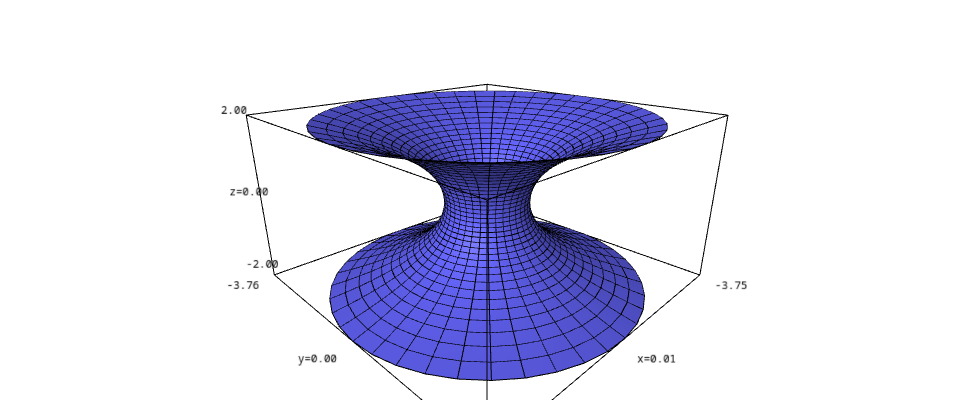
\includegraphics[scale=.5]{Images/ex1-1.png}
    \caption{Hiperboloide}
    \label{fig:ex1-1}
\end{figure}
\end{ex}

\begin{definition}[Atlas]
Uma coleção de parametrizações que cobrem uma superfície S é dita \textbf{atlas de S} e cada uma das parametrizações é dita uma \textbf{carta}.
\end{definition}

\begin{ex}[Um atlas para a esfera]
Uma esfera não pode ser coberta por uma única parametrização, porem podemos cobrir ela com 2 parametrizações da seguinte forma

\begin{lstlisting}
# Define the parameterizations
esfera1(u, v) = (2 * u/(1  +u^2 + v^2), 
                 2 * v/(1 + u^2 + v^2), 
                 (u^2 + v^2 - 1)/(1 + u^2 + v^2))

esfera2(u, v) = (2 * u/(1  +u^2 + v^2), 
                 2 * v/(1 + u^2 + v^2), 
                 -(u^2 + v^2 - 1)/(1 + u^2 + v^2))

# Plot
E1 = parametric_plot3d(esfera1, (u, -1, 1), (v, -1, 1), 
                       mesh=True, color='white')

E2 = parametric_plot3d(esfera2, (u, -1, 1), (v, -1, 1), 
                       mesh=True, color='red')


show(E1 + E2)
\end{lstlisting}

\begin{figure}[H]
    \centering
    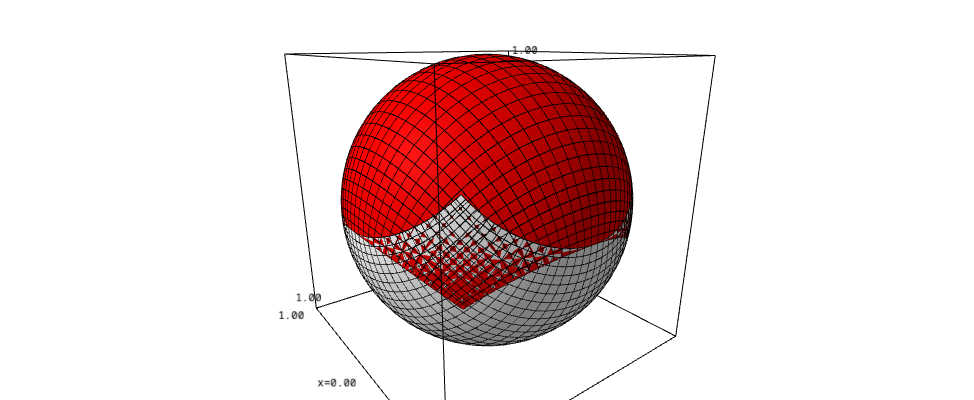
\includegraphics[scale=.5]{Images/ex1-2.png}
    \caption{Esfera com 2 parametrizações}
    \label{fig:ex1-2}
\end{figure}
\end{ex}

\begin{definition}[Curvas regulares enquanto subconjuntos]
Diz-se que um subconjunto $C \subset \mathbb{R}^3$ é uma \textbf{curva regular}, quando para cada $p \in C$, existe um intervalo aberto $I \subset \mathbb{R}$ e um difeomorfismo $\alpha: I \rightarrow \alpha(I) \subset C$ em que $\alpha(I)$ é um aberto relativo de C.
\end{definition}

\begin{definition}[Superfícies Regulares]
Um conjunto $S \subset \mathbb{R}^3$ é dito uma \textbf{superfície regular}, quando é localmente difeomorfo a $\mathbb{R}^2$. Mais precisamente, quando, $\forall p \in S$, exite um difeomorfismo

$$X: U \subset \mathbb{R}^2 \rightarrow V \subset S$$

onde U é um aberto de $\mathbb{R}^2$ e V é um aberto relativo de S. A aplicação X é dita, então uma parametrização local de S em p.
\end{definition}

\begin{ex}[Superfícies regulares]
Pela definição de superfície regular, temos que, as seguintes superfícies são regulares: plano, gráficos de funções de 2 variáveis, esferas, superfícies de revolução, etc.
\end{ex}

\begin{definition}
Sendo o difeomorfismo de uma superfície da forma

$$X(u, v) = (x(u, v), y(u, v), z(u, v)),\ (u,v) \in V$$

definimos as \textbf{derivadas parciais} de X como sendo

$$X_u(u, v) = \left( \frac{\partial x}{\partial u}(u, v), \frac{\partial y}{\partial u}(u, v), \frac{\partial z}{\partial u}(u, v) \right)$$

$$X_v(u, v) = \left( \frac{\partial x}{\partial v}(u, v), \frac{\partial y}{\partial v}(u, v), \frac{\partial z}{\partial v}(u, v) \right)$$

e se $X_u$ e $X_v$ são L.I. então produzem um plano tangente no ponto p.
\end{definition}

\begin{prop}
Se S é uma superfície regular temos que:

\begin{enumerate}[label=(\alph*)]
    \item A aplicação $X(u, v) = (x(u, v), y(u, v), z(u, v))$ é diferenciável de $C^\infty$ quando x, y e z tem derivadas parciais de todas as ordens.
    
    \item Para todo $q: (u, v) \in U$, a diferencial de X em q, $dX_q: \mathbb{R}^2 \rightarrow \mathbb{R}^3$ é injetiva, nesse caso, garante-se a existência do plano tangente $T_p S$.
\end{enumerate}
\end{prop}

\begin{theorem}[Função Inversa]
Seja F diferenciável e $p \in A$ tal que $dF_p$ é injetora. Então existe uma vizinhança $U \subset A$ de p. Tal que $F(U)$ é aberto em $\mathbb{R}^n$ e a restrição $F_U$ é um difeomorfismo de U sobre $F(U)$.
\end{theorem}

\begin{definition}[Valor Regular]
Dados um aberto $O \subset \mathbb{R}^3$ e uma função diferenciável $\varphi: O \rightarrow \mathbb{R}$. Dizemos que $q \in \mathbb{R}$ é \textbf{valor regular} de $\varphi$ quando $\forall p \in \varphi^-1(\{q\}) \subset O$ a derivada

$$d\varphi_p: \mathbb{R}^3 \rightarrow \mathbb{R}$$

é não nula, isto é, $\nabla \varphi(p) \neq 0$
\end{definition}

\begin{prop}
A \textbf{imagem inversa} de um valor regular de uma função diferenciável definida em um aberto do $\mathbb{R}^3$, quando não vazia, é uma superfície regular.
\end{prop}

\section*{Topologia}\label{s3}
\begin{definition}[Bola aberta]
Dado $a \in \mathbb{R}^n$ e um número real $r > 0$, a \textbf{bola aberta} de centro a e raio r em $\mathbb{R}^n$ é o conjunto

$$B(a, r) = \{ x \in \mathbb{R}^n\ |\ \| x - a \| \leq r \}$$

e respectivamente definimos \textbf{bola fechada} como

$$B(a, r) = \{ x \in \mathbb{R}^n\ |\ \| x - a \| \geq r \}$$
\end{definition}

\begin{definition}[Conjunto Limitado]
Um conjunto é dito \textbf{limitado} quando existe uma bola que o contém, ou seja,

$$\exists a \in \mathbb{R}^n\ \mathrm{e}\ r>0\ \mathrm{t.q.}\ X \subset B(a, r)$$
\end{definition}

\begin{definition}[Aplicação limitada]
Dado um conjunto A uma \textbf{aplicação} $f: A \rightarrow \mathbb{R}^n$ é dita limitada quando seu conjunto imagem é limitada.
\end{definition}

\begin{definition}[Conjunto aberto]
Um conjunto $A \subset \mathbb{R}^n$ é dito \textbf{aberto} quando $\forall a \in A \exists r > 0$ tal que $B(a, r) \subset A$ (e a é dito ponto interior de A).
\end{definition}

\begin{definition}[Aplicação aberta]
Diz-se que uma aplicação $f: \mathbb{R}^n \rightarrow \mathbb{R}^m$ é \textbf{aberta} quando $\forall A \subset \mathbb{R}^n\ \mathrm{aberto}, f(A) \subset \mathbb{R}^m$ é aberto.
\end{definition}

\begin{prop}[Propriedades dos abertos]
Propriedades fundamentais dos conjuntos abertos

\begin{enumerate}
    \item O conjunto vazio e o espaço $\mathbb{R}^n$ são abertos.
    
    \item A \textbf{intersecção} de uma família finita de abertos é aberta.
    
    \item A \textbf{união} de uma família qualquer de abertos é aberta.
\end{enumerate}
\end{prop}

\begin{definition}[Espaço topológico]
Um espaço topológico é um par $(X, T)$ em que X é um conjunto e T é uma família de subconjuntos de X, chamados abertos, que satisfazem as propriedades acima. Diz-se, então, que a família T define uma topologia
\end{definition}

\begin{theorem}
Uma sequência $(X_k)$ em $\mathbb{R}^n$ converge para $a \in \mathbb{R}^n$ se, e somente se, $\forall r > 0,\ \exists k_0 \in \mathbb{N}$ tal que se $k \geq k_0$ então $x_k \in B(a, r)$.
\end{theorem}

\begin{definition}[Conjunto fechado]
Um conjunto $F \subset \mathbb{R}^n$ é dito \textbf{fechado} quando seu complementar é aberto.
\end{definition}

\begin{prop}[Propriedades dos fechados]
Propriedades fundamentais dos conjuntos fechados

\begin{enumerate}
    \item O conjunto vazio e o espaço $\mathbb{R}^n$ são fechados.
    
    \item A \textbf{intersecção} de uma família qualquer de fechados é um conjunto fechado.
    
    \item A \textbf{união} de uma família finita de fechados é fechado.
\end{enumerate}
\end{prop}

\begin{definition}[Aplicação fechada]
Diz-se que uma aplicação $f: \mathbb{R}^n \rightarrow \mathbb{R}^m$ é \textbf{fechada} quando leva fechados de $\mathbb{R}^n$ em fechados de $\mathbb{R}^m$.
\end{definition}

\begin{definition}[Aderência]
Um ponto $a \in \mathbb{R}^n$ é dito \textbf{aderente} a um conjunto $X \subset \mathbb{R}^n$ se existe uma sequência de pontos de X que convergem para a.
\end{definition}

\begin{definition}[Fecho]
O \textbf{fecho} de X, denotado por $\overline{X}$, é o conjunto formado por todos os pontos de $\mathbb{R}^n$ que são aderentes a X.
\end{definition}

\begin{theorem}
$F \subset \mathbb{R}^n$ é fechado $\Longleftrightarrow \overline{F} = F$.
\end{theorem}

\begin{definition}[Bordo]
A fronteira (ou bordo) de um conjunto $X \subset \mathbb{R}^n$ é o conjunto $\partial X = \overline{X} \cap \overline{\mathbb{R}^n - X}$.
\end{definition}

\begin{definition}[Aberto relativo]
Sejam X subconjunto de $\mathbb{R}^n$ e $A \subset X$. Diz-se que A é \textbf{aberto relativo} a X ou \textbf{aberto relativamente} à X quando existe um aberto $U \subset \mathbb{R}^n$ tal que $A = U \cap C$.
\end{definition}

\begin{definition}[Cisão]
Uma \textbf{cisão} de um conjunto $X \subset \mathbb{R}^n$ é uma decomposição do mesmo em dois conjuntos disjuntos que são ambos, abertos em X, isto é, $A, B \subset \mathbb{R}^n$ tais que

\begin{itemize}
    \item $X = A \cup B$
    
    \item $A \cap B = \O$
    
    \item A e B abertos em X
\end{itemize}
\end{definition}

\begin{definition}[Conexidade]
Um conjunto $X \subset \mathbb{R}^n$ é dito \textbf{conexo} se a única cisão que admite é a trivial ($X = X \cup \O$) caso contrario é dito desconexo.
\end{definition}

\begin{definition}[Homeomorfismo]
Diz-se que dois espaços $(X_1, T_1)$ e $(X_2, T_2)$. São \textbf{homeomorfos} quando existe bijeção $\varphi: X_1 \rightarrow X_2$ tal que para quaisquer abertos $A_1 \in T_1$ e $A_2 \in T_2$ tem-se que $\varphi(A_1) \in T_2$ e $\varphi^{-1}(A_2) = T_1$. Logo $\varphi$ é dito \textbf{homeomorfismo}.
\end{definition}

\begin{definition}[Continuidade]
Dados $X, Y \subset \mathbb{R}^n$, $f: X \rightarrow Y$ é \textbf{contínua} em $a \in X$ se $\forall \varepsilon > 0,\ \exists \delta > 0$ tal que $x \in X$ e $\| x - a \| < \delta \Rightarrow \| f(x) - f(a) \| < \varepsilon$.
\end{definition}

\begin{theorem}
Dados $X \subset \mathbb{R}^n$ e $Y \subset \mathbb{R}^m$ uma bijeção $f: X \rightarrow Y$ é um homeomorfismo se e só se f e $f^{-1}$ são continuas.
\end{theorem}

\begin{definition}[Isomorfismo]
É uma aplicação que preserva uma estrutura e pode ser revertida com uma aplicação inversa.
\end{definition}

\section*{Primeira Forma Fundamental}\label{s4}

\bibliographystyle{sbc}
\bibliography{referencias}

\end{document}
